%! TeX program = lualatex
\documentclass[main]{subfiles}

\begin{document}

\title[AutoML: BO]{Acquisition Functions}
\subtitle{Bayesian Surrogate Models and Lower Confidence Bound}
\author[Bernd Bischl]{Bernd Bischl}
\date{}

\titlebackground*{images/AutoML_HPO_2_2}

    \maketitle


% \begin{frame}[t]{Bayesian Surrogate Modeling}
%   \begin{itemize}
%   \end{itemize}
%   \vfill
%   \begin{center}
%     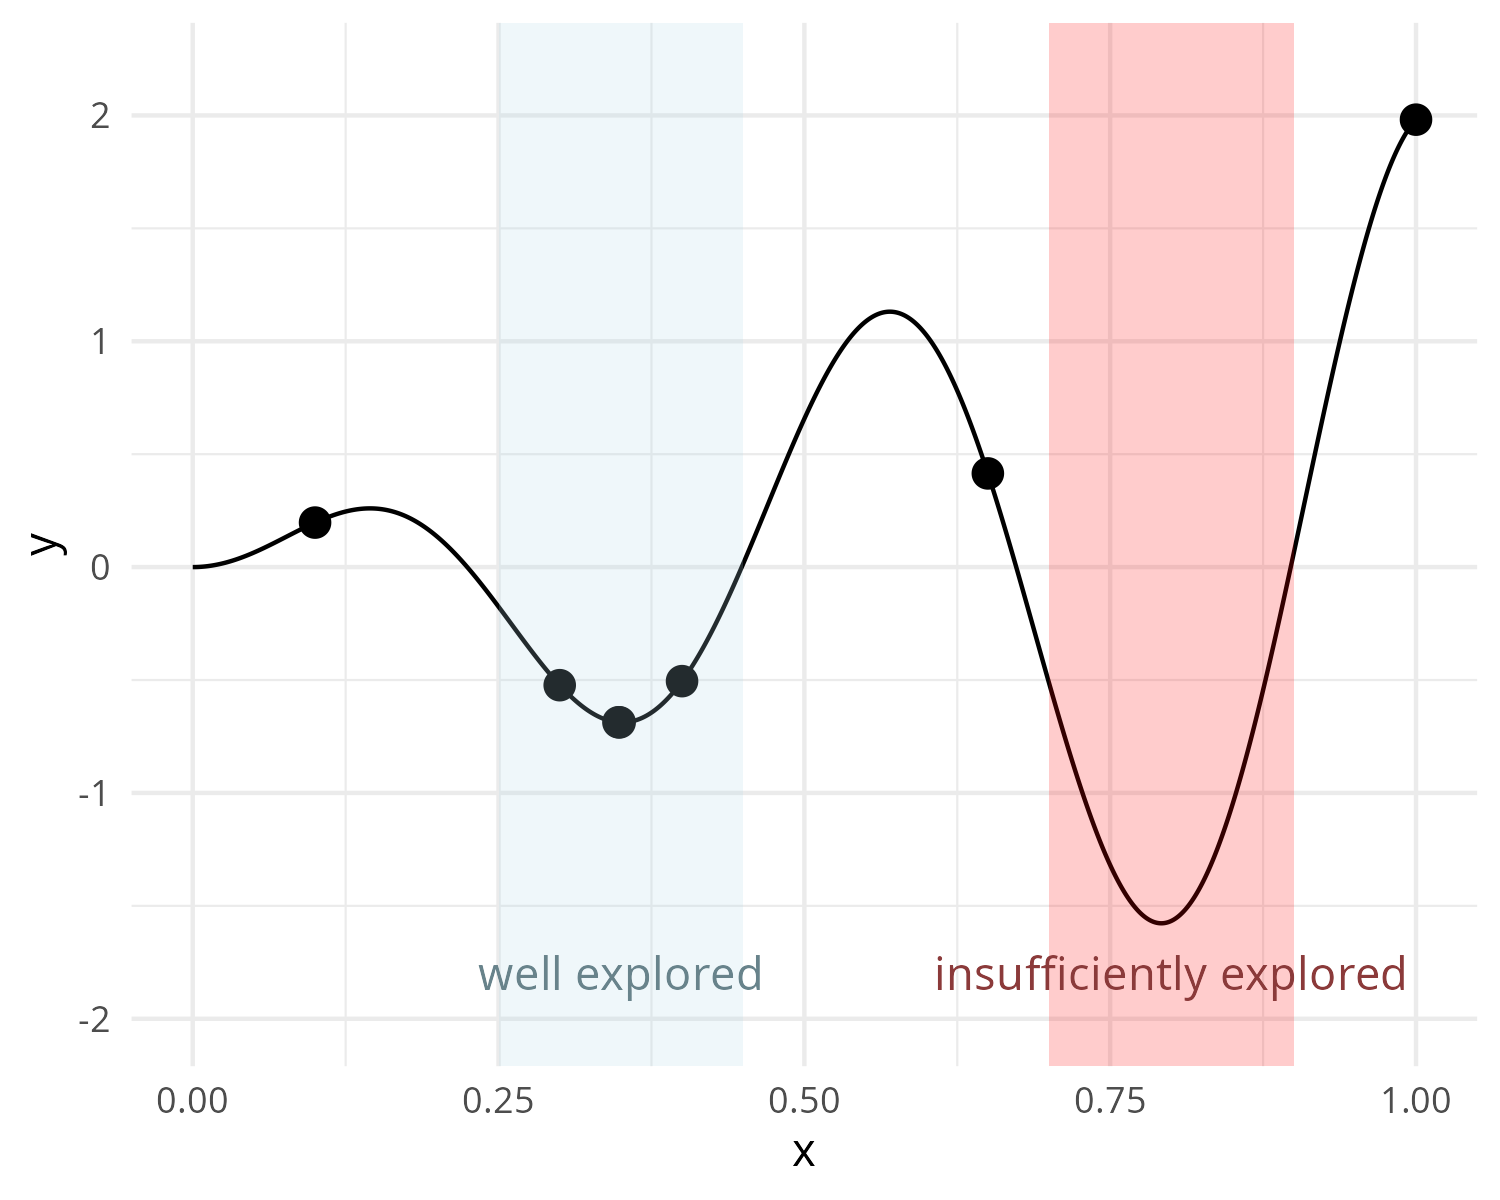
\includegraphics[width=.6\textwidth]{images/bayesian_loop_ee.png}
%   \end{center}
% \end{frame}


\begin{frame}[t]{Bayesian Surrogate Modeling}
  \small
  \begin{itemize}
    \item \textbf{Goal:} Find a trade-off between \textbf{exploration} (areas we have not visited yet) and \textbf{exploitation} (search around good design points)
    \item \textbf{Idea:} Use a \textbf{Bayesian approach} to build a surrogate model yielding estimates for the posterior mean $\surro(\conf)$ and posterior variance $\sh^2(\conf)$
    \item $\sh^2(\conf)$ expresses ``confidence''/``certainty'' in the prediction
    % \item To sequentially propose new points based on the surrogate model, we use \textbf{acquisition functions} $a: \pcs \to \R$
    % \item Let $\fmin := \min\{\cost(\confI{1}), \ldots, \cost(\confI{t})\}$ be the best observed value so far (green in plots)
    % \item In the examples before, we simply used the posterior mean $\acq(\conf) = \surro(\conf)$ as acquisition function -- ignoring uncertainty
  \end{itemize}
  \vfill
  \begin{columns}[onlytextwidth]
    \column{.5\textwidth}
    \begin{center}
      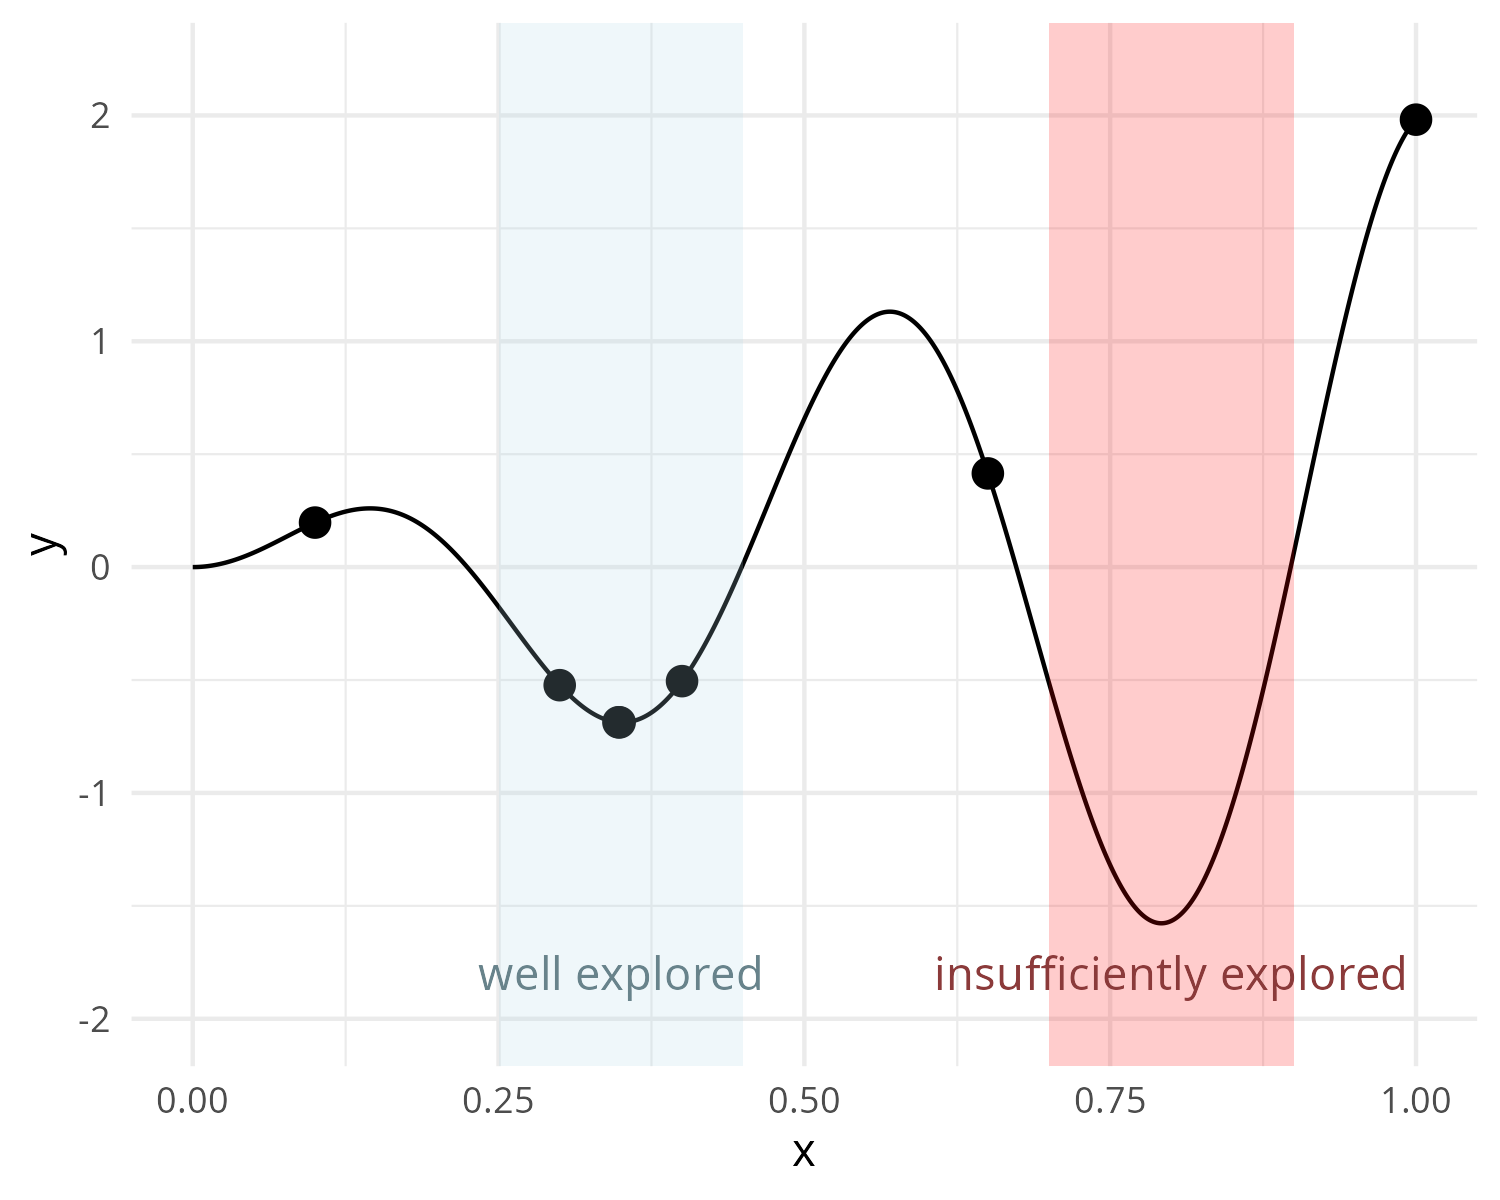
\includegraphics[width=0.6\textwidth]{images/bayesian_loop_ee.png}
    \end{center}
    \column{.5\textwidth}
    \begin{center}
      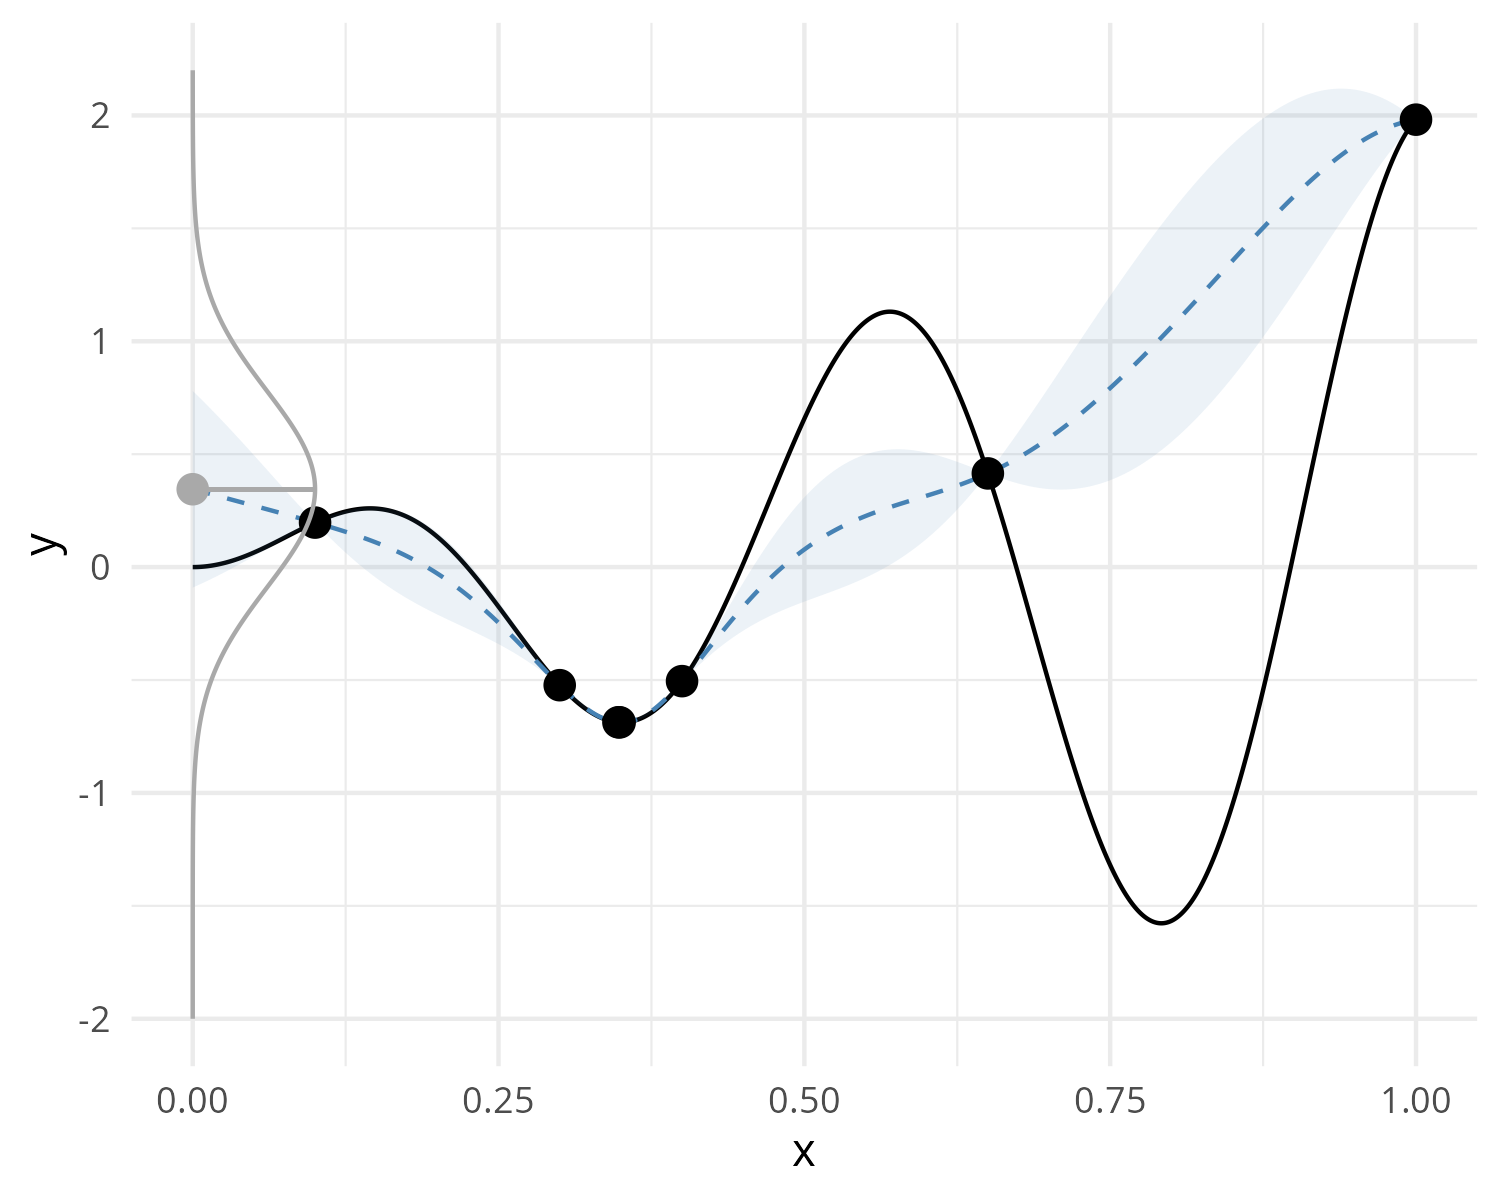
\includegraphics[width=0.6\textwidth]{images/bayesian_loop_sm_normal.png}
    \end{center}
  \end{columns}
\end{frame}


% \begin{frame}[t]{Bayesian Surrogate Modeling}
%   \begin{itemize}
%     \item Denote by $Y \mid \conf, \hist$ the (conditional) random variable associated with the posterior predictive of a new point $\conf$ under the surrogate model; abbreviated $Y(\conf)$
%     \item Most prominent choice: a \textbf{Gaussian process}, here $Y(\conf) \sim \normal\left(\surro(\conf), \sh^2(\conf)\right)$
%     \item For now we assume an interpolating SM; $\surro(\conf) = \cost(\conf)$ and $\sh(\conf) = 0$ at training points
%   \end{itemize}
%   \vfill
%   \begin{center}
%   \end{center}
% \end{frame}


\begin{frame}[t]{Acquisition Functions}
  \begin{itemize}
    \item To sequentially propose new points based on the surrogate model, we use \textbf{acquisition functions} $a: \pcs \to \R$
    % \item Let $\fmin := \min\{\cost(\confI{1}), \ldots, \cost(\confI{t})\}$ be the best observed value so far (green in plots)
    \item In the examples before, we simply used the posterior mean $\acq(\conf) = \surro(\conf)$ as acquisition function -- ignoring uncertainty
  \end{itemize}
  \vfill
  \begin{columns}[onlytextwidth]
    \column{.5\textwidth}
    \begin{center}
      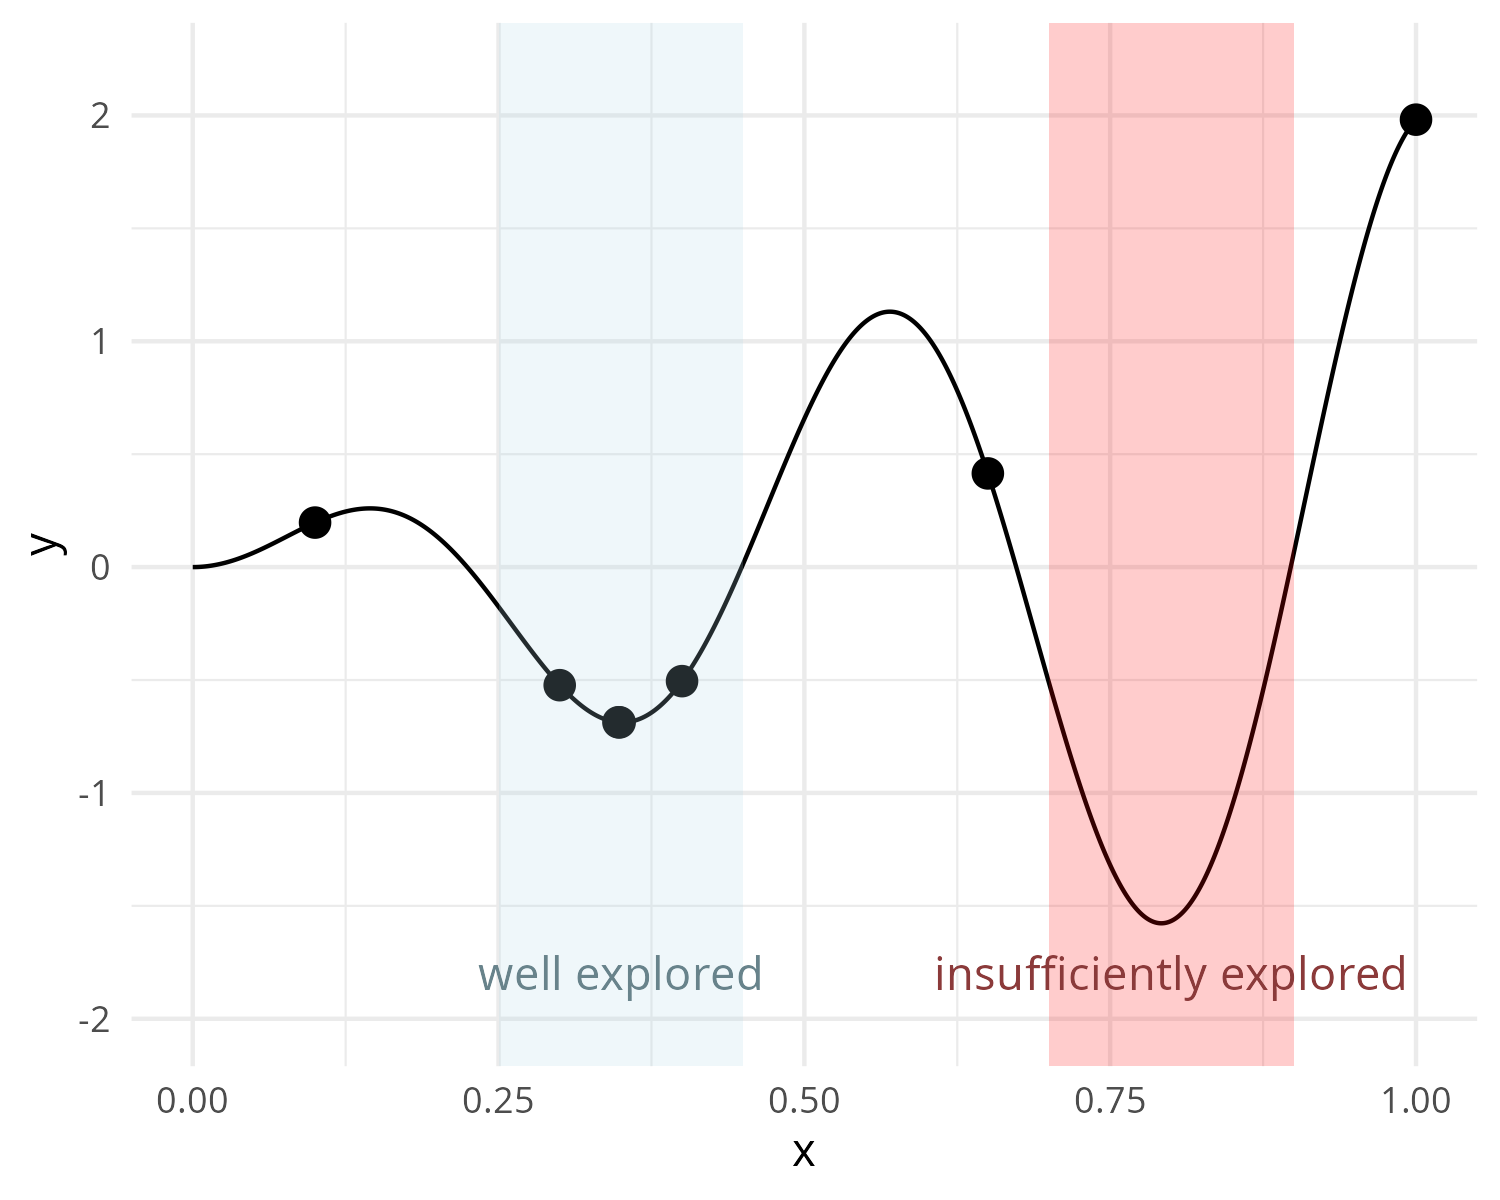
\includegraphics[width=0.6\textwidth]{images/bayesian_loop_ee.png}
    \end{center}
    \column{.5\textwidth}
    \begin{center}
      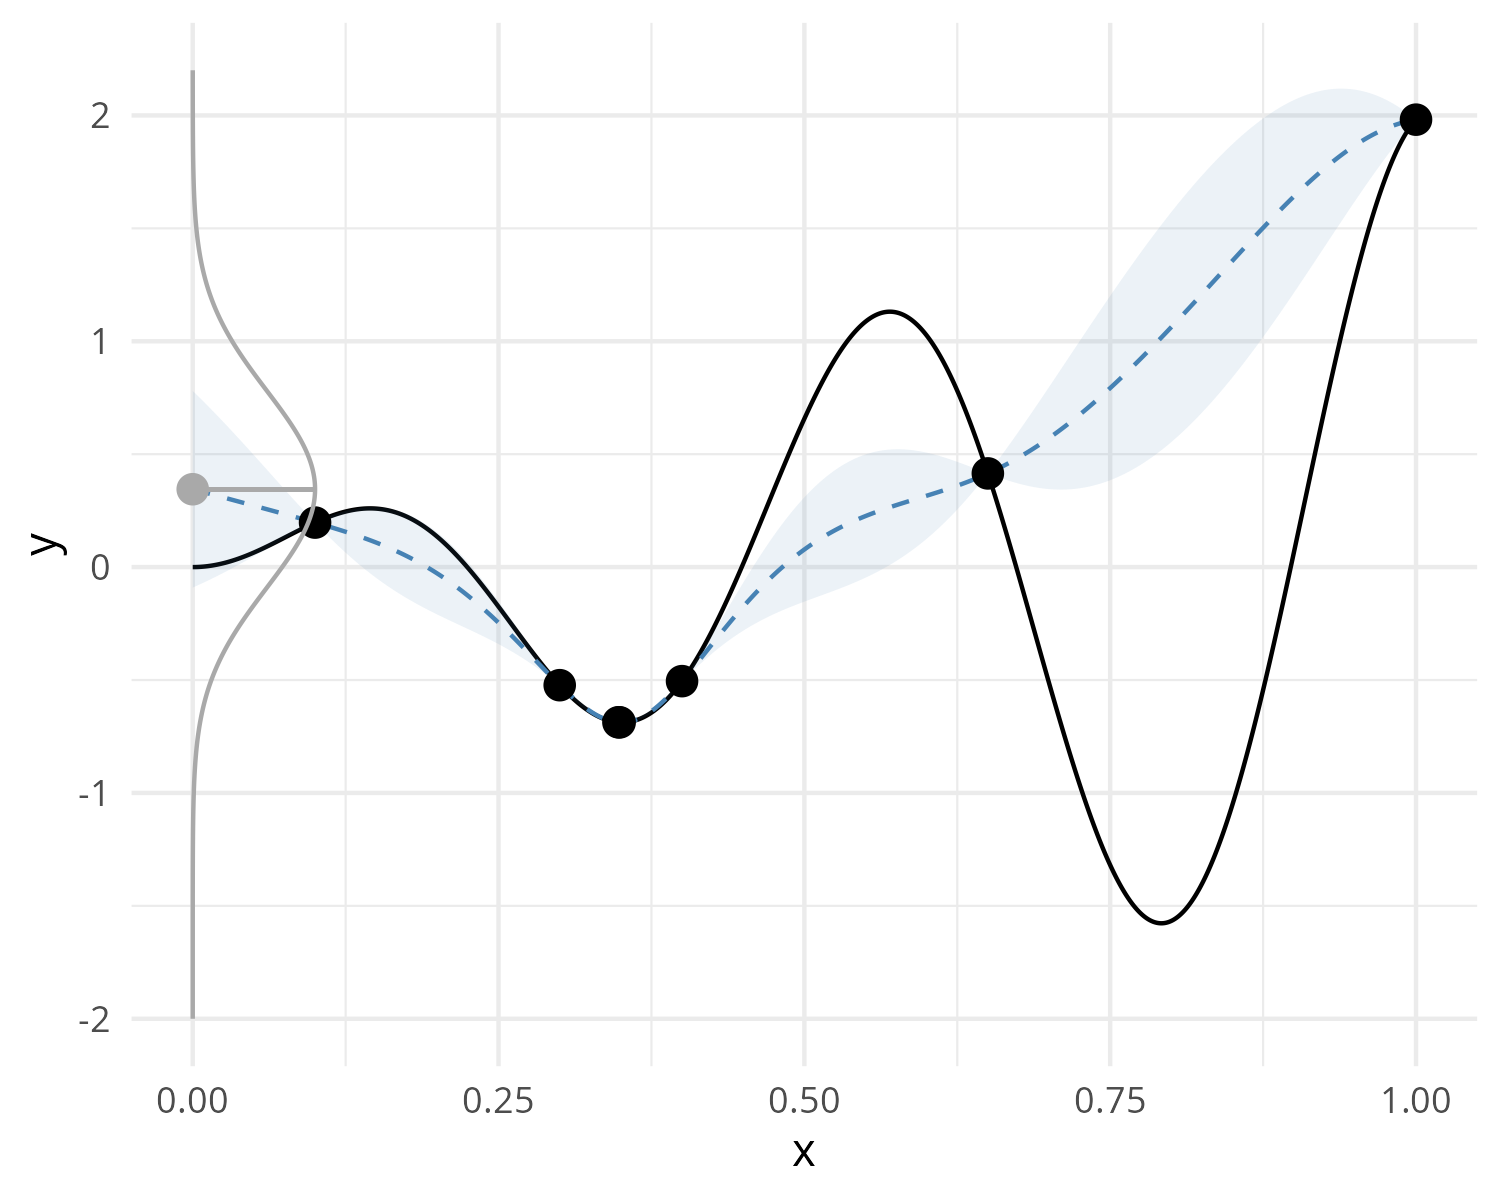
\includegraphics[width=0.6\textwidth]{images/bayesian_loop_sm_normal.png}
    \end{center}
  \end{columns}
\end{frame}


\begin{frame}[t]{Lower Confidence Bound}
  \begin{itemize}
    \item \textbf{Goal:} Find $\confI{t+1}$ that minimizes the \textbf{Lower Confidence Bound} (LCB):
    $$\acq_{\text{LCB}}(\conf) = \surro(\conf) - \tau \sh(\conf)$$
    where $\tau > 0$ controls the ``mean vs.\ uncertainty'' trade-off
    \item LCB is conceptually very simple
    \item Does \textbf{not} rely on distributional assumptions on the posterior predictive
  \end{itemize}
  \vfill
  \begin{center}
    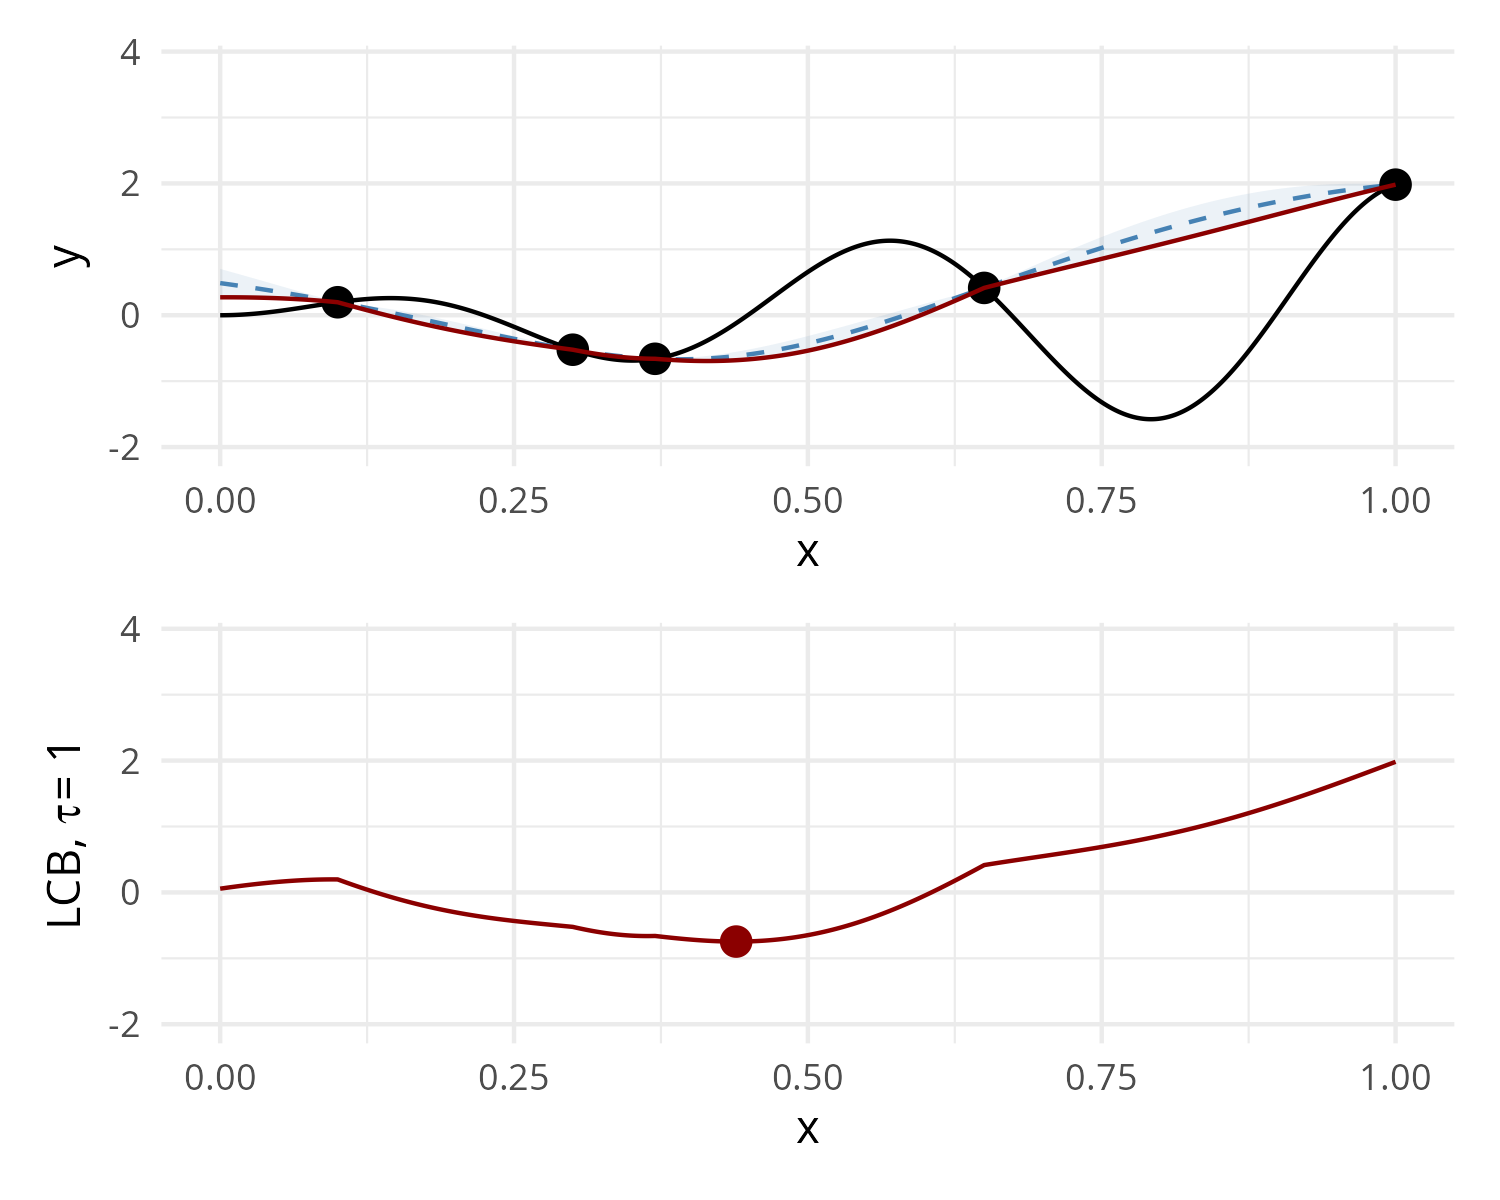
\includegraphics[width=.3\textwidth]{images/bayesian_loop_lcb_0.png}
  \end{center}
\end{frame}


\begin{frame}[t]{Probability of Improvement}
  \begin{itemize}
    \item \textbf{Goal:} Find $\confI{t+1}$ that maximizes the \textbf{Probability of Improvement} (PI):
    $$\acq_{\text{PI}}(\conf) = \P(Y(\conf) < \fmin) = \Phi\!\left(\frac{\fmin - \surro(\conf)}{\sh(\conf)}\right)$$
    where $\Phi(\cdot)$ is the standard normal cdf (assuming Gaussian posterior)
    \item PI does not take the size of the improvement into account
    \item Often proposes points close to the current $\fmin$
  \end{itemize}
  \vfill
  \begin{columns}[onlytextwidth]
    \column{.5\textwidth}
    \begin{center}
      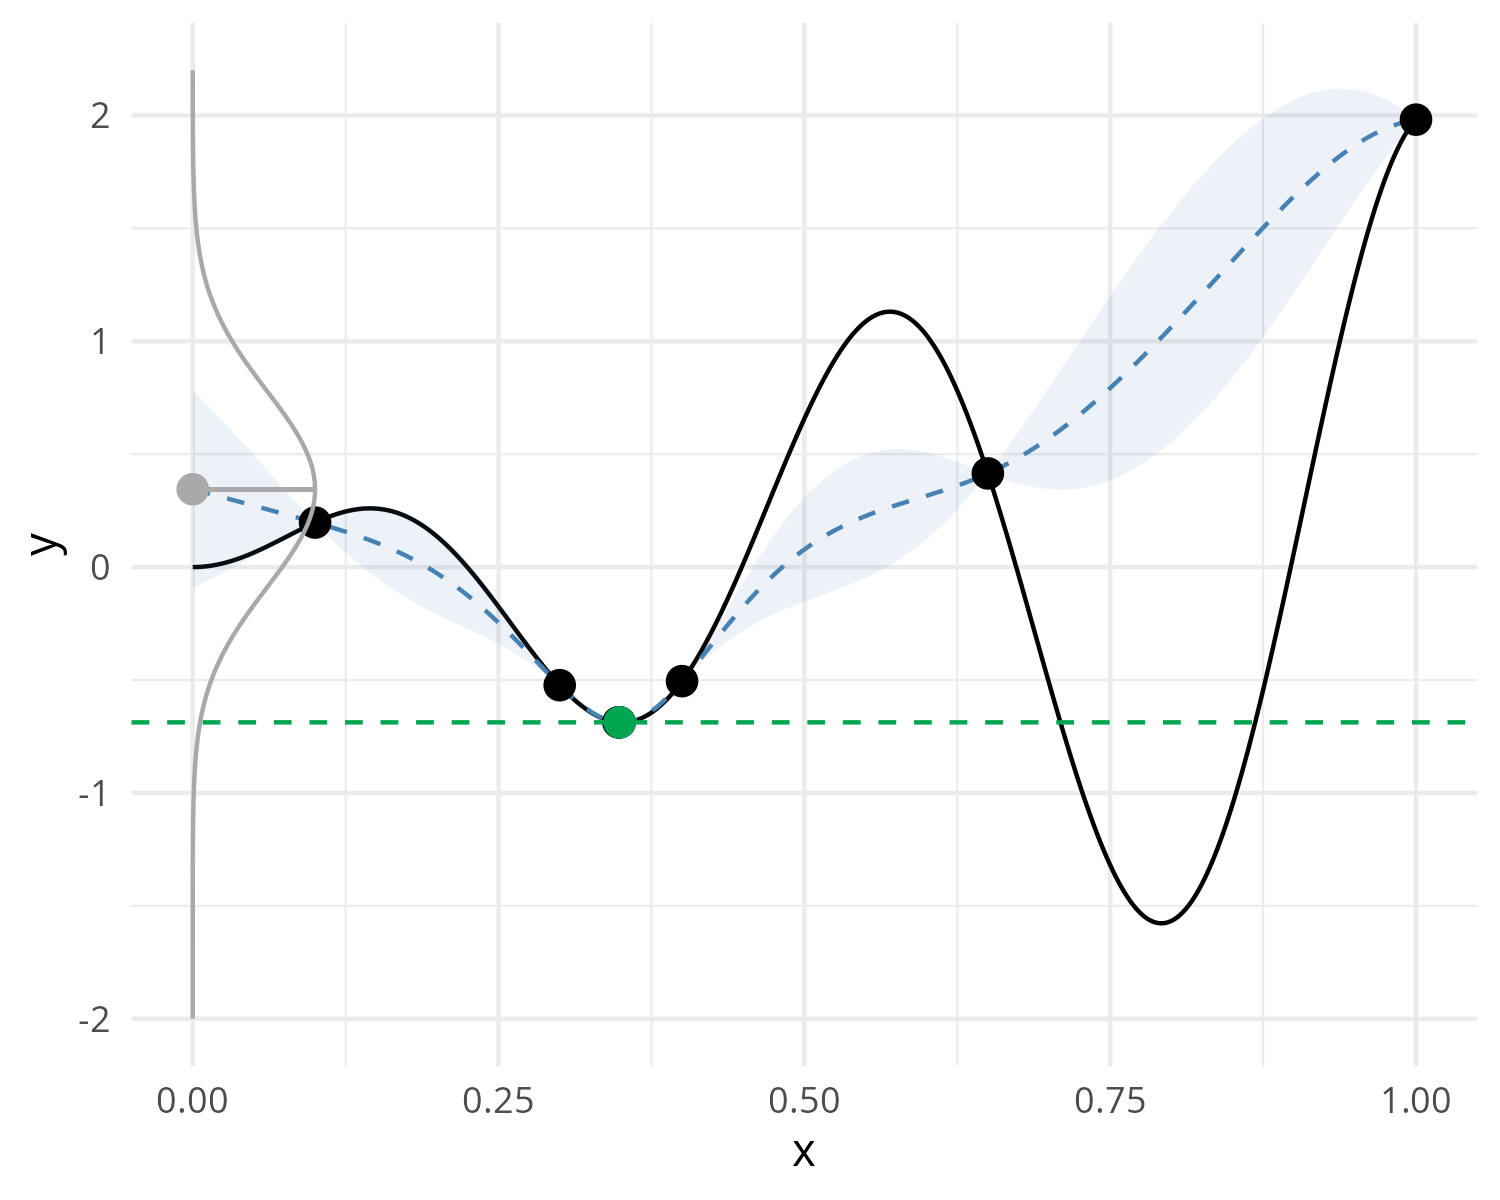
\includegraphics[width=\textwidth]{images/bayesian_loop_sm_normal_fmin.png}
    \end{center}
    \column{.5\textwidth}
    \begin{center}
      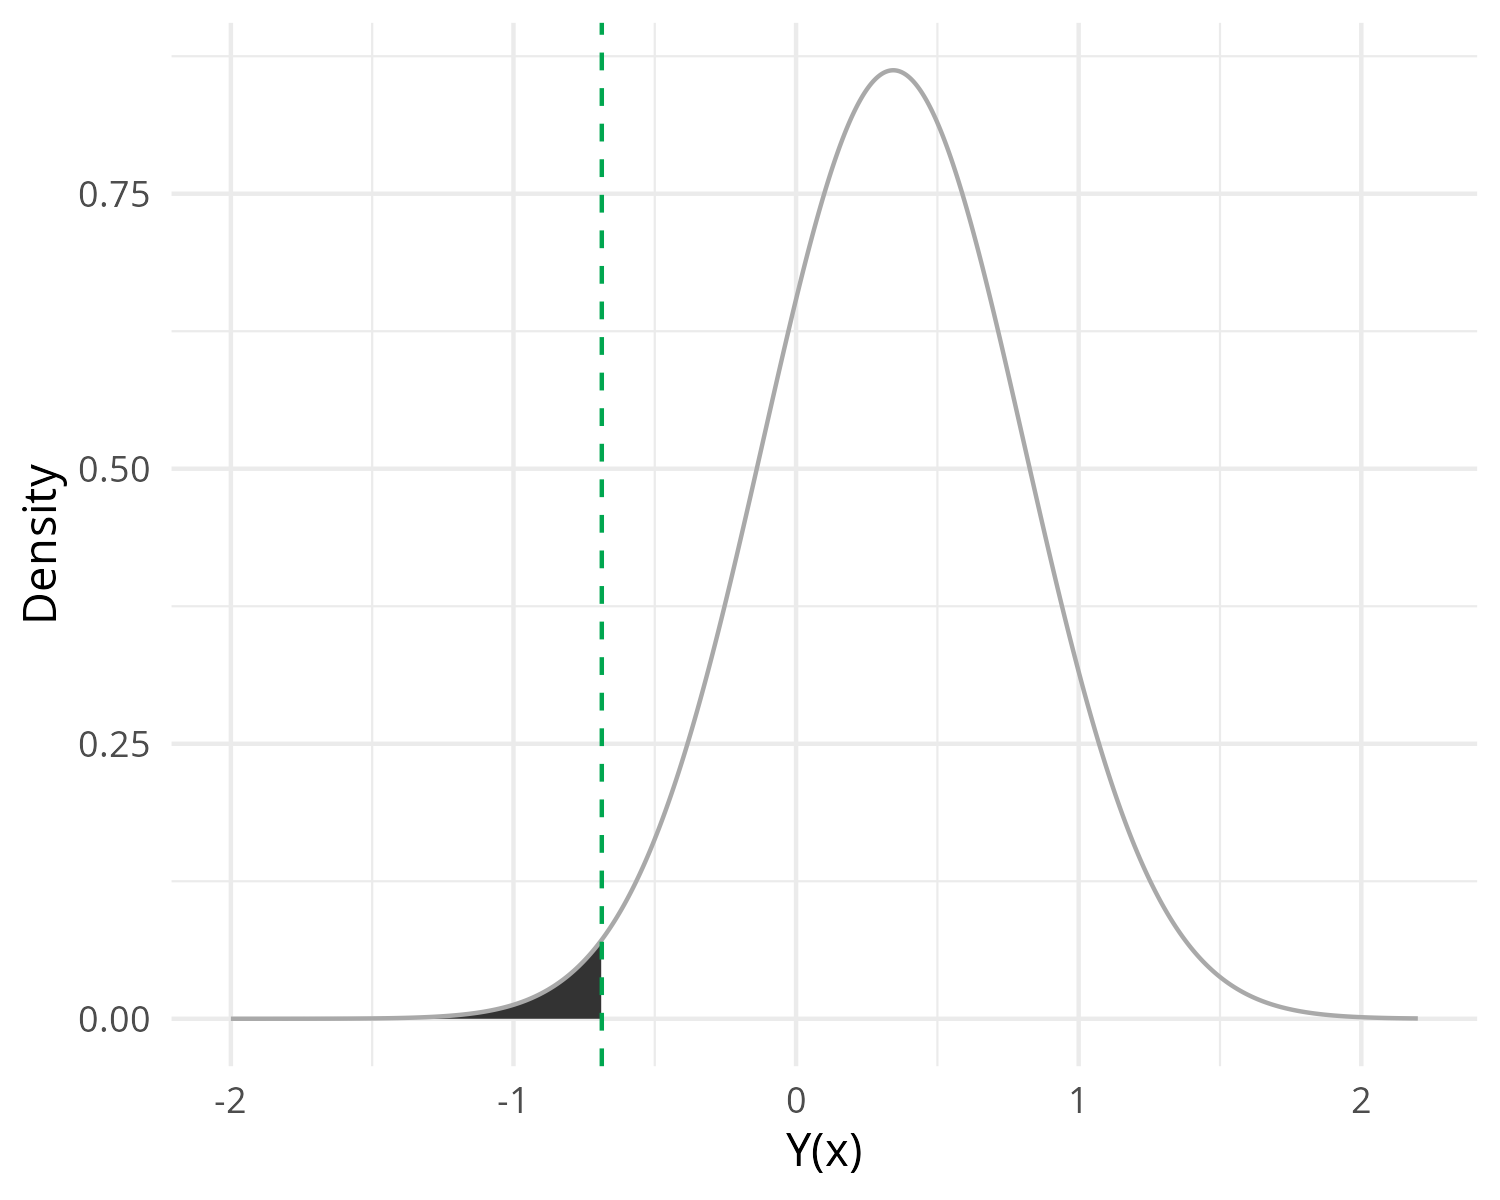
\includegraphics[width=\textwidth]{images/bayesian_loop_pi_0.png}
    \end{center}
  \end{columns}
\end{frame}


\begin{frame}[t]{Expected Improvement}
  \begin{itemize}
    \item \textbf{Goal:} Propose $\confI{t+1}$ that maximizes the \textbf{Expected Improvement} (EI):
    $$\acq_{\text{EI}}(\conf) = \E(\max\{\fmin - Y(\conf), 0\})$$
    \item We take the \emph{expectation} in the tail, instead of the probability as in PI
    \item Improvement is always assumed $\geq 0$
  \end{itemize}
  \vfill
  \begin{columns}[onlytextwidth]
    \column{.5\textwidth}
    \begin{center}
      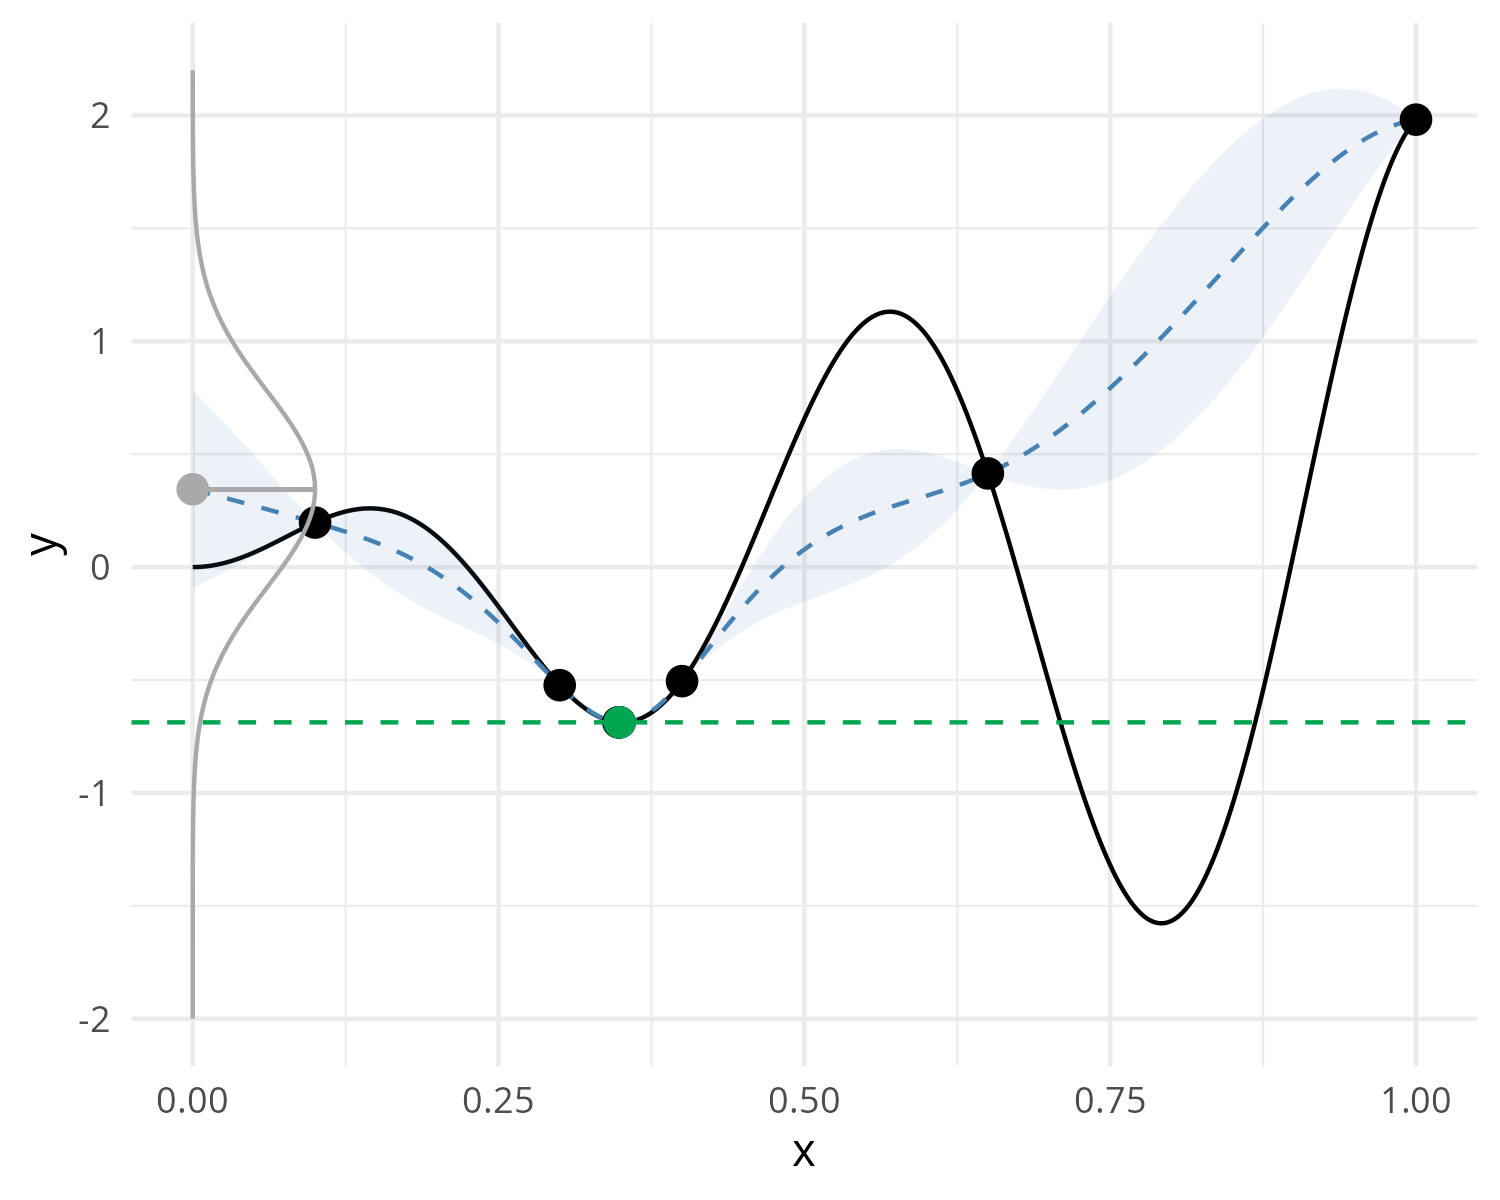
\includegraphics[width=\textwidth]{images/bayesian_loop_sm_normal_fmin.png}
    \end{center}
    \column{.5\textwidth}
    \begin{center}
      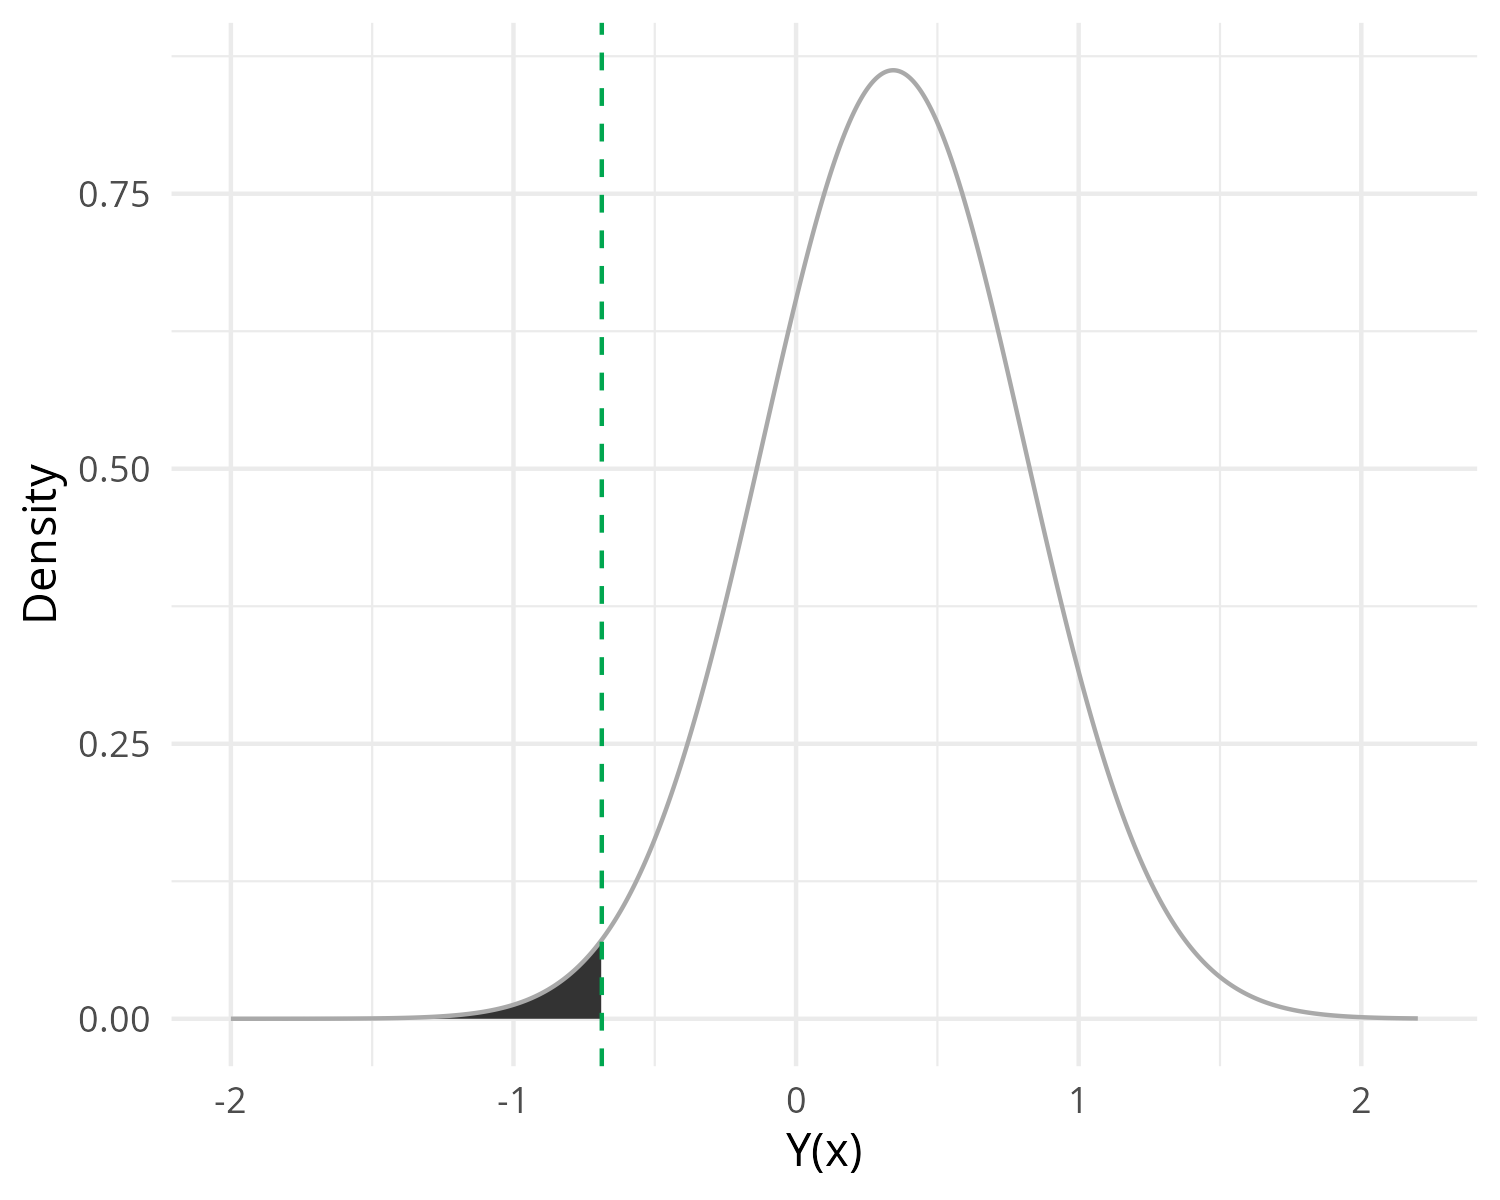
\includegraphics[width=\textwidth]{images/bayesian_loop_pi_0.png}
    \end{center}
  \end{columns}
\end{frame}


\begin{frame}[t]{Expected Improvement}
  \begin{itemize}
    \item If $Y(\conf) \sim \normal\left(\surro(\conf), \sh^2(\conf)\right)$, the EI has a closed form:
    $$\acq_{\text{EI}}(\conf) = (\fmin-\surro(\conf))\, \Phi\!\left(\frac{\fmin - \surro(\conf)}{\sh(\conf)}\right) + \sh(\conf)\, \phi\!\left(\frac{\fmin - \surro(\conf)}{\sh(\conf)}\right)$$
    \item $\acq_{\text{EI}}(\conf) = 0$ at design points:
    $$\acq_{\text{EI}}(\conf) = (\fmin-\surro(\conf)) \underbrace{\Phi\!\left(\tfrac{\fmin - \surro(\conf)}{\sh(\conf)}\right)}_{= 0, \text{ see PI}} + \underbrace{\sh(\conf)}_{= 0}\, \phi\!\left(\tfrac{\fmin - \surro(\conf)}{\sh(\conf)}\right)$$
  \end{itemize}
\end{frame}


\begin{frame}[t]{Expected Improvement}
  \begin{itemize}
    \item EI is capable of exploration and quickly proposes promising points in areas we have not visited yet
    \item Here, also a result of the well-calibrated uncertainty $\sh(\conf)$ of our GP
  \end{itemize}
  \vfill
  \begin{center}
    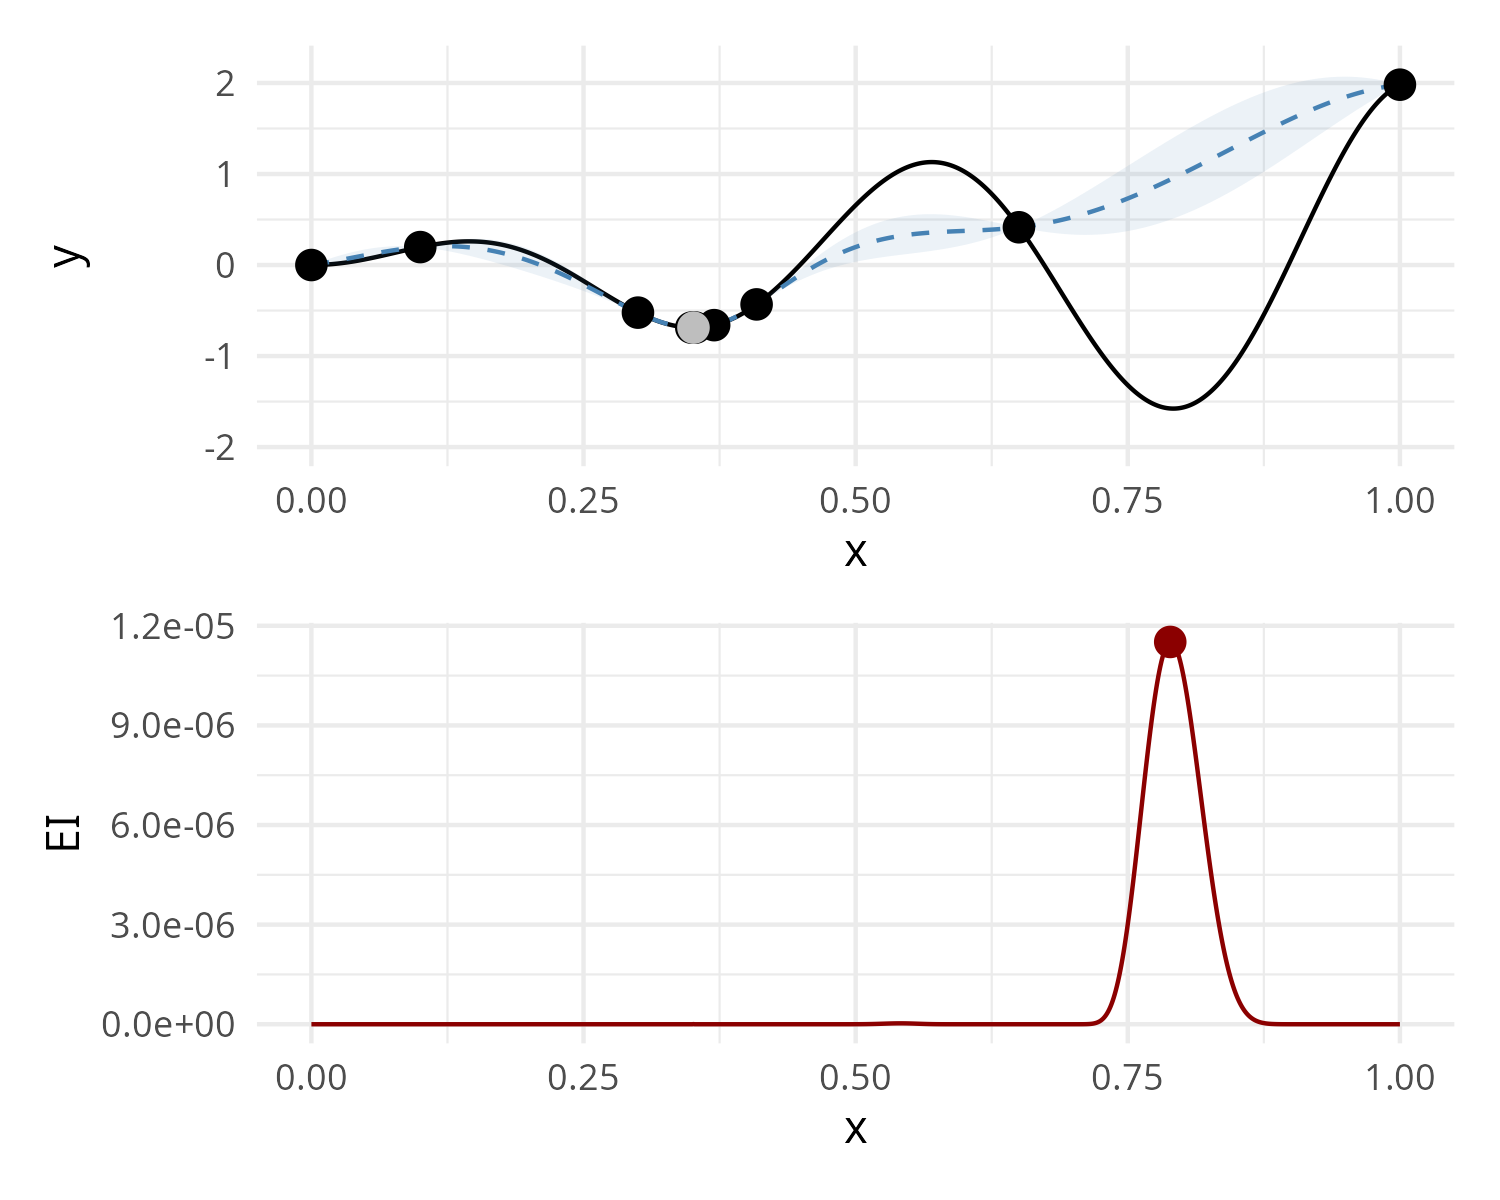
\includegraphics[width=.7\textwidth]{images/bayesian_loop_6.png}
  \end{center}
\end{frame}


\begin{frame}[t]{Summary and Discussion}
  \begin{itemize}
    \item ACQFs balance exploitation and exploration, usually by combining posterior mean and uncertainty
    \item 3 basic ACQFs: PI, LCB, EI
    \item EI is most standard; LCB also works well in practice
    \item Under some mild conditions: BO with a GP as SM and EI is a \textbf{global optimizer}, i.e.\ convergence to the \textbf{global} optimum is guaranteed given unlimited budget~\liturl{Bull 2011}{https://www.jmlr.org/papers/volume12/bull11a/bull11a.pdf}
    \item Other acquisition functions: Entropy Search, Predictive Entropy Search, Max-value Entropy Search, Knowledge Gradient, Thompson Sampling, \ldots
  \end{itemize}
\end{frame}


\end{document}
